\documentclass{beamer}
\usepackage[polish]{babel}
\usepackage[utf8]{inputenc}
\usepackage[T1]{fontenc}
\usepackage{hyperref}

\usetheme[progressbar=frametitle]{metropolis}
\setbeamertemplate{frame numbering}[fraction]
\useoutertheme{metropolis}
\useinnertheme{metropolis}
\usefonttheme{metropolis}
\usecolortheme{spruce}
\setbeamercolor{background canvas}{bg=white}


\definecolor{green}{rgb}{.125,.5,.25}
\usecolortheme[named=green]{structure}

\title{Prezentacja przy użyciu klasy Beamer}
\author{Karol Lewandowski}
\date{30 stycznia 2022}

\begin{document}
\metroset{block=fill}

\begin{frame}
\titlepage
\end{frame}

\begin{frame}[t]{Funkcje} \vspace{4pt}
\begin{block}{Definicja funkcji}
\vspace{0.5em}
\textbf{Funkcję} definiuje się jako przyporządkowanie każdemu elementowi jednego zbioru, dokładnie jednego elementu drugiego zbioru.
\vspace{0.5em}
\end{block}

\begin{figure}[h!]
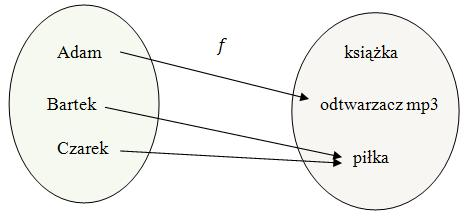
\includegraphics[scale=0.4]{funkcja.png}
\caption{przykład funkcji}
\end{figure}

\end{frame}

\begin{frame}[t]{Funkcje - przykłady} \vspace{4pt}
\begin{block}{Definicja funkcji wykładniczej}
\vspace{0.5em}
\textbf{Funkcja wykładnicza} ma wzór: f(x) = $a^{x}$, gdzie $a$ > 0. Nazwa funkcji wykładniczej pochodzi od tego, że x znajduje się w wykładniku.
\vspace{0.5em}
\end{block}

\begin{figure}[h!]
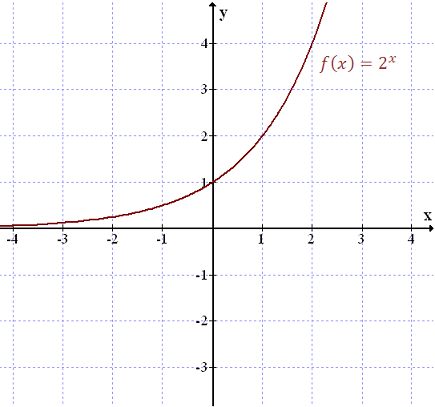
\includegraphics[scale=0.2]{funkcja2.png}
\caption{przykład funkcji wykładniczej}
\end{figure}

\end{frame}

\begin{frame}[t]{Funkcje - przykłady} \vspace{4pt}
\textbf{Definicje funkcji trygonometrycznych w trójkącie prostokątnym}

\begin{figure}[h!]
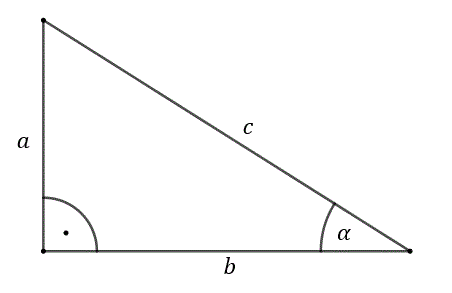
\includegraphics[scale=0.35]{funkcja3.png}
\end{figure}


{\small Boki $a$ oraz $b$ - to \textbf{przyprostokątne} trójkąta prostokątnego.}
\newline
{\small Bok $c$ - to \textbf{przeciwprostokątna} trójkąta prostokątnego.}


\begin{figure}[h!]
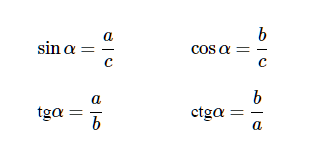
\includegraphics[scale=0.5]{funkcja4.png}
\end{figure}

\end{frame}

\begin{frame}[t]{Funkcje - przykłady} \vspace{4pt}
\begin{block}{Definicja pochodnej funkcji}
\textbf{Pochodna funkcji} - miara szybkości (tempa) zmian wartości funkcji względem jej argumentów.
\end{block}

\begin{figure}[h!]
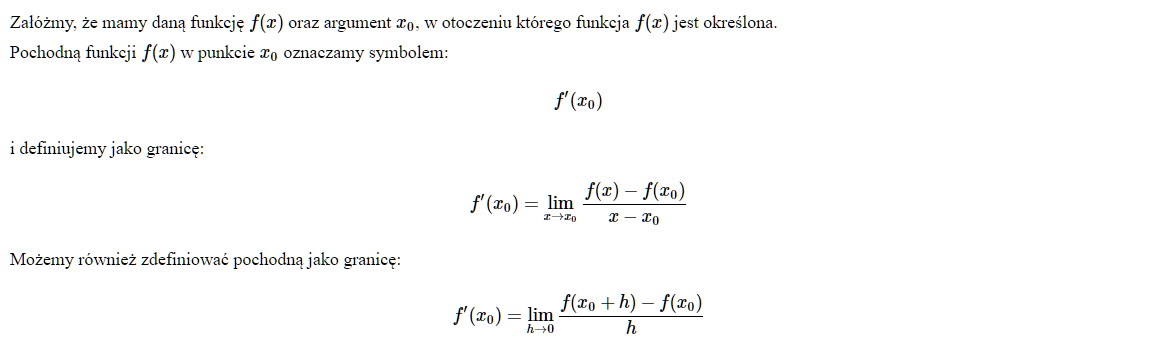
\includegraphics[scale=0.5]{funkcja5.png}

\end{figure}

\end{frame}

\begin{frame}[t]{Przebieg zmiennosci funkcji} \vspace{4pt}
\textbf{Badanie przebiegu zmiennosci funkcji}
\newline
Podczas badania przebiegu zmiennosci funkcji należy wyznaczyć:
\begin{enumerate} [1. ]
\item Dziedzinę.
\item Miejsca zerowe.
\item Punkt przecięcia z osią Oy.
\item Granice na krańcach dziedziny.
\item Asymptoty.
\item Przedziały monotoniczności.
\item Ekstrema lokalne.
\end{enumerate}
Na końcu rysujemy wykres funkcji i odczytujemy z niego zbiór wartosci funkcji.
\end{frame}

\begin{frame}[t]{Przebieg zmiennosci funkcji} \vspace{4pt}
\textbf{Przykładowa tabela przebiegu zmiennosci funkcji}
\begin{center}
\begin{tabular}{ | c | c | c | c | c | c | c | c | }
\hline
x & (-$\infty$, -1) & -1 & (-1, 0) & 0 & (0, 1) & 1 & (1, +$\infty$) \\ 
\hline
f'(x) & - &  & - & - & - &  & - \\
\hline
f''(x) & - &  & + & 0 & - &  & + \\
\hline
f(x) & 0 $\nearrow$ -$\infty$ &  & +$\infty$ $\searrow$ 0 & 0 p.p. & 0 $\nearrow$ -$\infty$ &  & +$\infty$ $\searrow$ 0 \\
\hline
\end{tabular}
\end{center}
\end{frame}

\begin{frame}[t]{Równania kwadratowe}
\textbf{Proste równania kwadratowe}
\newline
Najprostszymi równaniami kwadratowymi są równania typu:
\begin{figure}[h!]
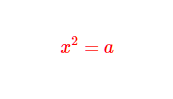
\includegraphics[scale=0.7]{zdj2.png}
\end{figure}
\begin{figure}[h!]
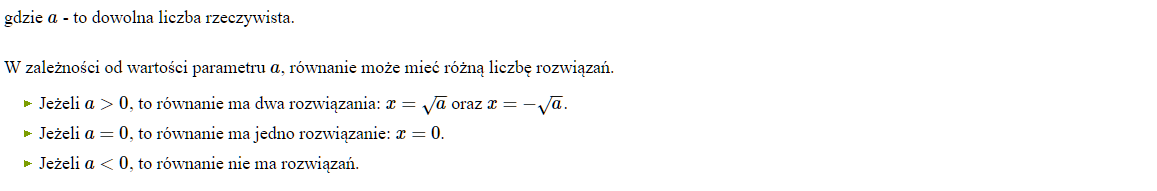
\includegraphics[scale=0.5]{zdj3.png}
\end{figure}
\end{frame}

\begin{frame}[t]{Nierównosci kwadratowe} \vspace{4pt}
\textbf{Metoda rozwiązywania nierównosci kwadratowych}
\newline
Metodę rozwiązywania nierówności kwadratowej można zapisać w czterech krokach:
\begin{enumerate} [a) ]
\item wszystkie wyrazy przenosimy na lewą stronę nierówności, tak aby po prawej zostało tylko 0,
\item lewą stronę nierówności traktujemy jako wzór funkcji kwadratowej,
\item wyznaczamy miejsca zerowe tej funkcji kwadratowej (o ile istnieją) i szkicujemy jej wykres,
\item odczytujemy z wykresu rozwiązanie nierówności.
\end{enumerate}
\end{frame}

\begin{frame}[t]{Netografia i bibliografia} \vspace{4pt}
Bibliografia:
\begin{enumerate} [1. ]
\item\url{https://www.matemaks.pl/metoda-rozwiazywania-nierownosci-kwadratowych.html}
\item\url{https://www.matemaks.pl/pochodne.html}
\item\url{https://www.matemaks.pl/funkcje-definicje-i-wlasnosci.html}
\end{enumerate}

\begin{figure}[h!]

\includegraphics[scale=0.1]{zdj.png}
\end{figure}

\end{frame}

\end{document}